%%%%%%%%%%%% FORMATO DE LA REVISTA MOMENTO %%%%%%%%%%%%%%%%%

% En el directorio de trabajo deben estar los archivos: momento (tipo LaTeX Class), articulo (tipo LaTeX Class), éstos archivos no se deben modificar,  Bibfile (tipo BibTex Database) en donde el autor debe introducir los datos de las referencias en formato BibTex y  Formato.tex (éste archivo en donde se edita el contenido del documento


%-----------------------------------------------------
%PAQUETES
\documentclass{momento}
\usepackage[pdftex]{graphicx}
\usepackage{verbatim}
\usepackage[centerlast,sc,footnotesize]{caption}
\usepackage{subfigure}
\usepackage{amsmath}
\usepackage[spanish, es-tabla]{babel} %Idioma español
\usepackage[utf8]{inputenc} %Acentos español
%--------------------------------------------------

%%%%%%%%%%% TITULO DEL ARTICULO (Los títulos, resúmenes y palabras clave se organizan dependiendo del idioma en el que se escriba el artículo. Entonces, si el artículo se escribe en español se debe colocar primero el título en español y luego en inglés. Si el artículo se escribe en inglés se coloca primero el título en inglés y luego en español. Así mismo para el resumen y palabras clave)
\title{TITULO DEL ARTÍCULO EN ESPAÑOL\\[0.5cm]
TITULO DEL ARTÍCULO EN INGLES}

%%%%%%%%%%% AUTORES DEL ARTICULO
\author{Autor I\suprm1, Autor II \suprm2 }
% Por cada autor \suprm# es para referenciar la afiliacion del autor con el número #. Se debe incluir de cada autor el primer nombre, inicial del segundo nombre si lo tiene y el primer apellido. 

%%%%%%%%%%% INSTITUCION DE LOS AUTORES
\newcommand{\afiliacion}{\suprm 1 Afiliación autor I \\ \suprm 2 afiliación autor II }
% Escribir afiliación (Grupo de investigación, Dependencia, Universidad, País) de los autores dentro del corchete derecho. 
% Recuerde que el caracter \\ es para comenzar una nueva linea

%%%%%%%%%%% ENCABEZADOS
\newcommand{\autor}{Autor I y Autor II}
\newcommand{\tema}{Título corto del artículo}
% Autor 1 y Autor 2         -----> aparecen en el encabezado de las paginas pares
% Titulo corto del articulo -----> aparece en el encabezado de las paginas impares


%%%%%%%%%%% CORREOS ELECTRONICOS DE LOS AUTORES
\authorinfo{e-mail de contacto}
%A1 y A2 son las iniciales del nombre de los autores correspondientes

%%%%%%%%%%% PAGINA EN QUE COMIENZA EL ARTICULO (RESERVADO PARA EL EDITOR)
\setcounter{page}{1}

%%%%%%%%%% Estilo de la bibliografia segun la American Physics Society 
\bibliographystyle{apsrev4-1}
\begin{document}
\maketitle

%%%%%%%%%%% RESUMEN DE SU ARTICULO EN ESPAÑOL
\begin{resumen}
    \noindent Escribir resumen en español.
\end{resumen}

%%%%%%%%%%% PALABRAS CLAVE DE SU ARTICULO EN ESPAÑOL
\keywords{Palabras clave en español.}

%%%%%%%%%%% RESUMEN DE SU ARTICULO EN INGLÉS
\begin{ingles}
    \noindent Escribir resumen en inglés
\end{ingles}
%%%%%%%%%%% PALABRAS CLAVE DE SU ARTICULO EN INGLÉS
\ikeywords{Palabras clave en inglés.}

%%%%%%%%%%% CUERPO DEL DOCUMENTO
% El texto debe dividirse en secciones, cada una con un encabezado (por ejemplo: Introducción; Parte Experimental, Materiales y Métodos o Desarrollo teórico; Resultados; Discusión; Conclusiones). Se recomienda que estas secciones sean breves y equilibradas.
\subsection*{Introducción}

\noindent Comienzo del cuerpo del artículo.\\

\noindent Las referencias citadas aquí son ejemplos de cómo se debe referenciar un artículo \cite{1}, un libro \cite{2}, una conferencia \cite{3}, una página web \cite{4} y memorias de congreso \cite{5}. \\

\noindent Las figuras deben tener buena resolución (mínimo 300 pixeles por pulgada) en escala de grises o a color de ser estrictamente necesario.  Al graficar diferentes series de datos usar en lo posible diferentes símbolos (marcadores de datos en excel), como se muestra en la fig. \ref{figura1}.

\begin{figure}
    \begin{center}
        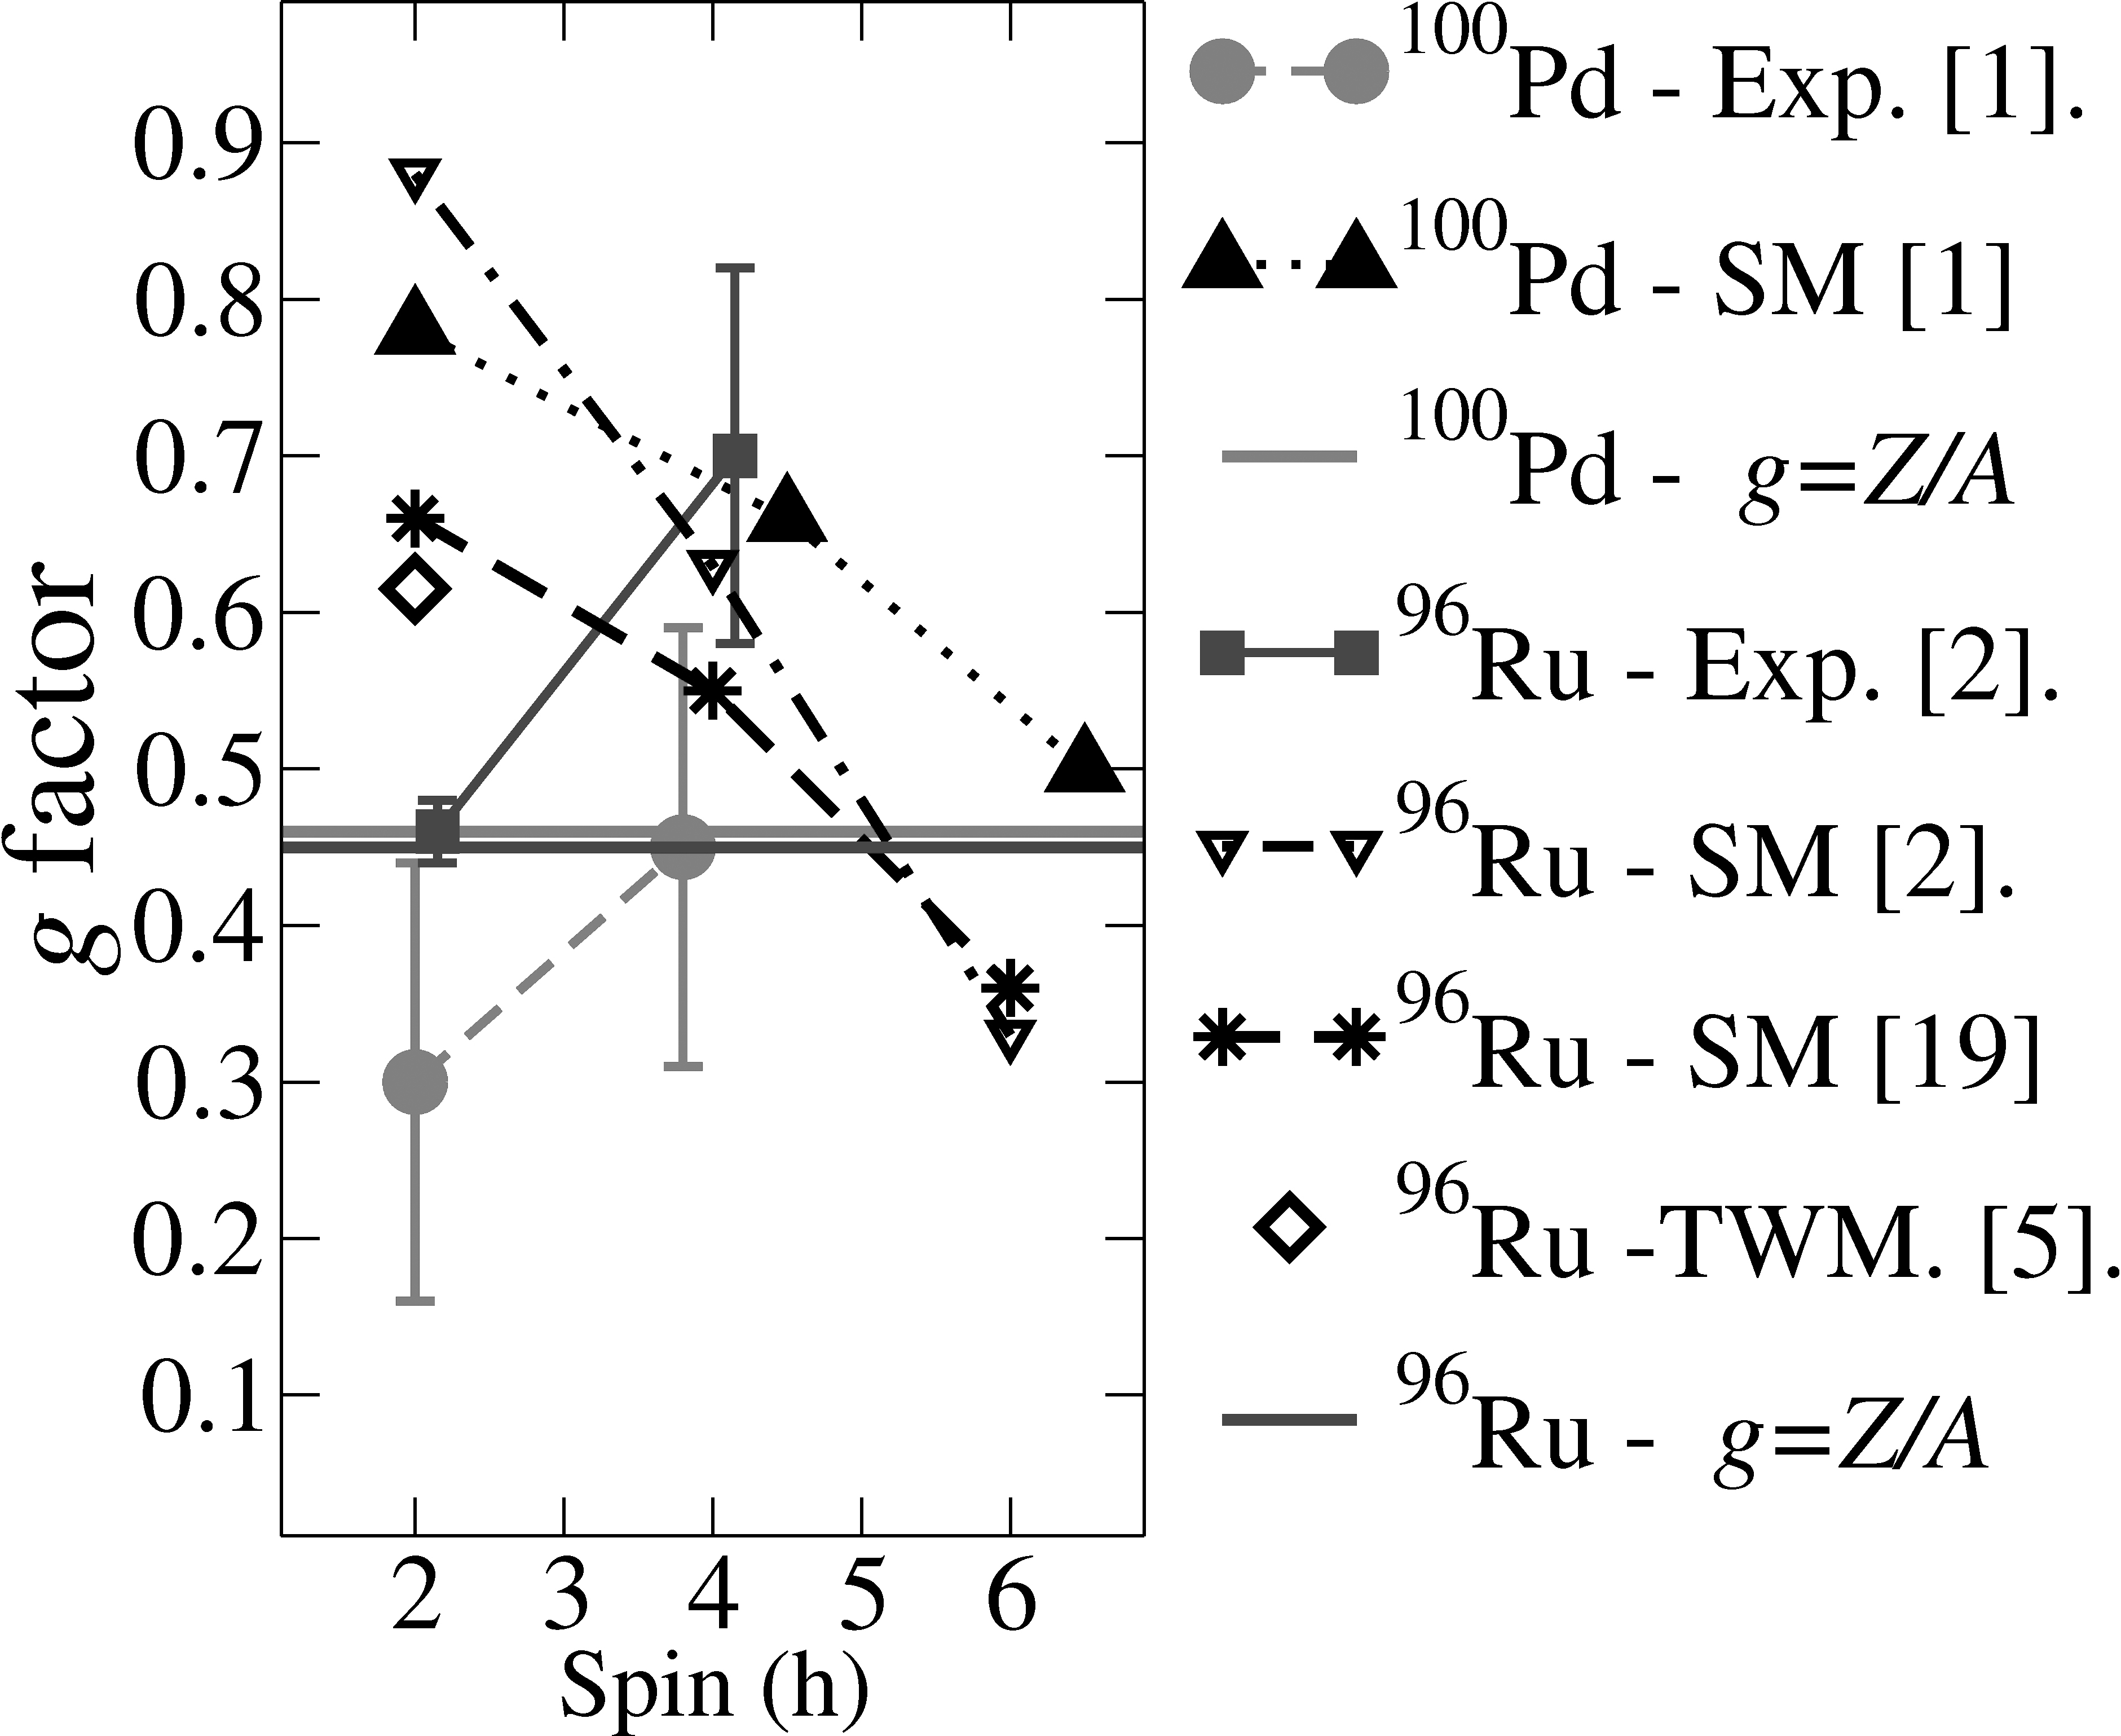
\includegraphics[width=7cm]{figura1.jpg}
    \end{center}
    \caption{\itshape Ejemplo figura.}
    \label{figura1}
\end{figure}

\noindent - Unidades, abreviaturas y símbolos: Se usará el Sistema Internacional de Unidades (m, kg, s, K), empleando sólo términos aceptados generalmente. Es necesario explicar las abreviaturas desconocidas cuando se usen por primera vez. Se debe poner especial cuidado al escribir los símbolos para que sean identificados claramente. En casos especiales, se especificará directamente con el autor el uso de fórmulas, caracteres especiales u otros.

%%%%Otras secciones pueden ser incluidas usando el comando subsection

\subsection*{Conclusiones}
Conclusiones del artículo

%- Si se requieren agradecimientos, reconocimientos a entidades, permisos de publicación, etc., irán al terminar el texto y antes de las Referencias bibliográficas.

%archivo tipo bib donde se encuentran las referencias
\bibliography{bibfile}

\end{document}



